\documentclass[12pt]{article}

% Paquetes básicos primero
\usepackage[utf8]{inputenc}
\usepackage[T1]{fontenc}
\usepackage{ragged2e}
\usepackage[spanish]{babel}

% Geometría y diseño
\usepackage{geometry}
\geometry{
	letterpaper,
	left=2.5cm,
	right=2.5cm,
	top=3cm,
	bottom=3cm,
	headheight=60pt,
	headsep=1cm
}

% Paquetes de formato
\usepackage{setspace}
\usepackage{graphicx}
\usepackage{fancyhdr}
\usepackage{xcolor}
\usepackage{enumitem}
\usepackage{lastpage}
\usepackage{background}
\usepackage{textcomp}

% Paquetes para referencias
\usepackage[round]{natbib}  % Configuración específica para citas
\bibliographystyle{plainnat}  % Estilo de bibliografía

% URLs y enlaces (hyperref debe ir al final)
\usepackage{url}
\usepackage[hidelinks]{hyperref}

% Configuración del encabezado y pie de página
\pagestyle{fancy}
\fancyhf{}
\renewcommand{\headrulewidth}{0pt}
\renewcommand{\footrulewidth}{0pt}

\definecolor{tecnmBlue}{RGB}{0, 43, 89}
\definecolor{tecnmWhite}{RGB}{255, 255, 255}

% Definir comandos para reducir la carga
\newcommand{\smallgray}[1]{{\scriptsize\textcolor{gray}{#1}}}

\fancyhead[L]{%
	\hspace*{0.5cm}\raisebox{-2.2\height}{
\includegraphics[height=1cm]{imagenes/logotecnm.png}}%
}

\fancyhead[R]{%
	\raisebox{-1.7\height}{%
		\begin{tabular}[b]{r}
			{\scriptsize\textbf{Instituto Tecnológico de Morelia}}\\[-0.6em]
			\smallgray{Subdirección Académica}\\[-0.6em]
			\smallgray{Departamento de Sistemas y Computación}\\[-0.6em]
			\smallgray{Internet de las Cosas}\\[-0.4em]
			{\scriptsize Página \thepage\ de \pageref{LastPage}}
		\end{tabular}%
	}%
}

\makeatletter
\renewcommand\@biblabel[1]{#1.}
\makeatother

\fancyfoot[L]{%
	\small
	Tarea 2
	
	\vspace{0.1cm}
	
	\small\textcolor{gray}{Equipo 1}
}

\fancyfoot[R]{%
	\small
	\textbf{Sensor Ultrasonico}%
}

% Definir comando para citas
\newcommand{\cita}[1]{\cite{#1}}

\begin{document}
	\pagenumbering{arabic}
	
	
	% Secciones principales
	% portada.tex
% Configuración del fondo solo para la portada
\backgroundsetup{
	scale=1,
	angle=0,
	opacity=0.2,
	contents={
\includegraphics[width=\paperwidth,height=\paperheight]{imagenes/fondo_portada.png}}
}
\BgThispage

\begin{center}
	\vspace*{2cm}
	
	\Large\textbf{Actividad 1: Led y Boton de encendido y apagado}
	
	\vspace{1.5cm}
	
	Autor(es):
	
	\vspace{0.5cm}
	
	Luis Fernando Chávez Martínez
	
	Luis Javier Ramírez Arias
	
	Mario Eduardo Sánchez Mejía
	
	
	\vspace{1.5cm}
	
	Docente:
	
	\vspace{0.5cm}
	
	
	Juan Jesús Ruiz Lagunas
	
	\vspace{0.5cm}
	
	\begin{abstract}
		\noindent
		\justifying
		Esta actividad consiste en el control de un LED mediante un botón utilizando una Raspberry Pi. Se implementa un sistema de encendido y apagado que permite al usuario interactuar con el LED a través del botón, utilizando los pines GPIO de la Raspberry Pi. Se abordan conceptos básicos de electrónica, como el uso de resistencias pull-up y pull-down, y se desarrolla un script en Python para gestionar la lógica de funcionamiento. Esta práctica permite familiarizarse con la manipulación de hardware en sistemas embebidos y su aplicación en proyectos de automatización.
		
		\vspace{0.5cm}
		\noindent
		\textbf{Palabras clave:} Raspberry Pi, GPIO, LED, botón, encendido/apagado, Python, electrónica básica, sistemas embebidos, automatización.
	\end{abstract}
\end{center}

% Desactivar el fondo para las siguientes páginas
\clearpage
\backgroundsetup{contents={}}
	\section{Introducción}
\noindent
\justifying
Los sensores ultrasónicos son ampliamente utilizados en aplicaciones de medición de distancia, detección de obstáculos y sistemas de navegación en robótica. El sensor HC-SR04 es un dispositivo de bajo costo que permite medir distancias mediante la emisión y recepción de ondas ultrasónicas, calculando el tiempo de retorno del eco para determinar la distancia a un objeto.

En esta práctica, se implementa un sistema de medición de distancia con un sensor HC-SR04 conectado a una Raspberry Pi. Se configura la comunicación a través de los pines GPIO y se emplea un divisor de voltaje para garantizar la compatibilidad entre la señal de retorno del sensor (5V) y los pines de la Raspberry Pi (3.3V). Se desarrolla un script en Python para enviar pulsos de activación al sensor, capturar la señal de respuesta y calcular la distancia en centímetros.

Este trabajo permite familiarizarse con la integración de sensores en sistemas embebidos, comprendiendo los principios básicos de la medición ultrasónica y su aplicación en proyectos de automatización, control de dispositivos y robótica. Además, refuerza el uso de la Raspberry Pi como una plataforma versátil para el desarrollo de soluciones tecnológicas.

	\newpage
	\section{Desarrollo}
\subsection{Materiales}
Para la implementación de este sistema de medición de distancia, se requieren los siguientes materiales:

\begin{itemize}
	\item Raspberry Pi 4 (o versión compatible)
	\item Sensor ultrasónico HC-SR04
	\item Protoboard
	\item Resistencias de 1 k\textohm{} y 2 k\textohm{} (para el divisor de voltaje)
	\item Cables de conexión (jumper)
	\item Fuente de alimentación para la Raspberry Pi (5V, 3A)
\end{itemize}

\subsection{Principio de funcionamiento}
El sensor HC-SR04 mide la distancia mediante la emisión de un pulso ultrasónico de 40 kHz a través de su pin \textit{Trig}. Este pulso viaja hasta un objeto y se refleja de vuelta al sensor, donde es recibido en el pin \textit{Echo}. La Raspberry Pi mide el tiempo transcurrido entre la emisión y recepción del pulso y, utilizando la velocidad del sonido en el aire (343 m/s), calcula la distancia con la siguiente ecuación:

\begin{equation}
	\mathrm{Distancia} = \frac{\mathrm{Tiempo\ de\ respuesta} \times 34300}{2}
\end{equation}

\subsection{Conexiones eléctricas}
Para conectar el sensor HC-SR04 a la Raspberry Pi, se utiliza el siguiente esquema:

\begin{itemize}
	\item \textbf{VCC} (HC-SR04) $\rightarrow$ \textbf{5V} (Raspberry Pi)
	\item \textbf{GND} (HC-SR04) $\rightarrow$ \textbf{GND} (Raspberry Pi)
	\item \textbf{Trig} (HC-SR04) $\rightarrow$ \textbf{GPIO 23} (Raspberry Pi)
	\item \textbf{Echo} (HC-SR04) $\rightarrow$ \textbf{Divisor de voltaje} $\rightarrow$ \textbf{GPIO 24} (Raspberry Pi)
\end{itemize}

\subsubsection{Divisor de voltaje}
Dado que el pin \textit{Echo} del HC-SR04 devuelve una señal de 5V y la Raspberry Pi solo soporta señales de 3.3V en sus pines GPIO, es necesario utilizar un divisor de voltaje con resistencias:

\begin{itemize}
	\item Conectar una resistencia de \textbf{1 k\textohm{}} entre el pin \textit{Echo} y el GPIO 24 de la Raspberry Pi.
	\item Conectar una resistencia de \textbf{2 k\textohm{}} entre el GPIO 24 y GND.
\end{itemize}

Este divisor reduce la señal de 5V a aproximadamente 3.3V, protegiendo la Raspberry Pi.

\subsection{Implementación en Python}
Para obtener la medición de distancia, se utiliza un script en Python que controla la activación del sensor y mide el tiempo de respuesta. A continuación, se presenta el código para la medición de distancia:

\begin{verbatim}
	import RPi.GPIO as GPIO
	import time
	
	# Definir pines
	TRIG = 23
	ECHO = 24
	
	# Configuración de pines
	GPIO.setmode(GPIO.BCM)
	GPIO.setup(TRIG, GPIO.OUT)
	GPIO.setup(ECHO, GPIO.IN)
	
	def medir_distancia():
	GPIO.output(TRIG, True)
	time.sleep(0.00001)
	GPIO.output(TRIG, False)
	
	while GPIO.input(ECHO) == 0:
	inicio = time.time()
	
	while GPIO.input(ECHO) == 1:
	fin = time.time()
	
	duracion = fin - inicio
	distancia = (duracion * 34300) / 2  # Velocidad del sonido: 343 m/s
	
	return distancia
	
	try:
	while True:
	distancia = medir_distancia()
	print(f"Distancia: {distancia:.2f} cm")
	time.sleep(1)
	except KeyboardInterrupt:
	GPIO.cleanup()
\end{verbatim}

\subsection{Ejecución del código}
Para ejecutar el código, se debe guardar el script como \texttt{ultrasonico.py} y ejecutarlo en la Raspberry Pi con el siguiente comando:

\begin{verbatim}
	python3 ultrasonico.py
\end{verbatim}

El programa imprimirá la distancia medida en centímetros cada segundo en la terminal.

\subsection{Aplicaciones y beneficios}
La integración del sensor HC-SR04 con la Raspberry Pi permite diversas aplicaciones, entre ellas:

\begin{itemize}
	\item Detección de obstáculos en robótica
	\item Medición de niveles en depósitos de líquidos
	\item Sistemas de asistencia para estacionamiento
	\item Sensores de proximidad en automatización industrial
\end{itemize}

Este proyecto permite comprender la medición ultrasónica y su aplicación en proyectos de control y automatización, reforzando la manipulación de hardware con Raspberry Pi.

\subsection{Fotografías de la Actividad}

\begin{figure}[h]
	\centering
	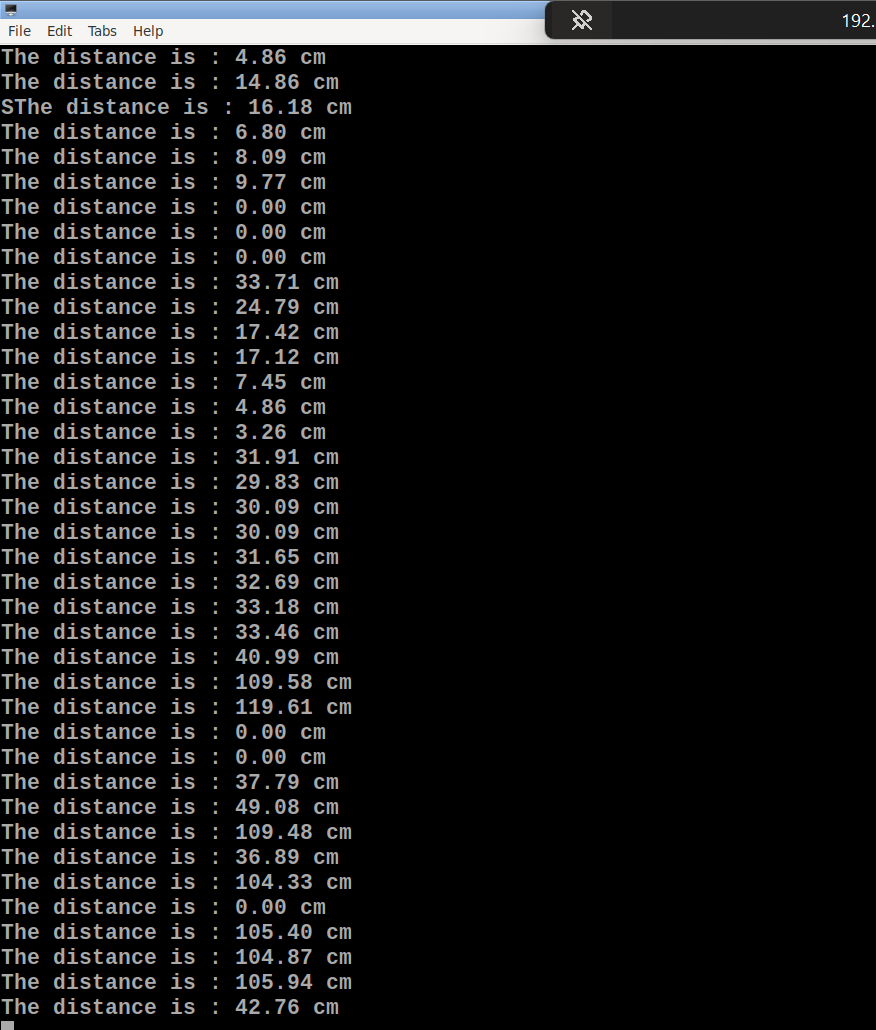
\includegraphics[width=0.5\textwidth]{imagenes/terminal}
	\caption{Foto de la terminal con las medidas del Ultrasónico}
\end{figure}

\begin{figure}[h]
	\centering
	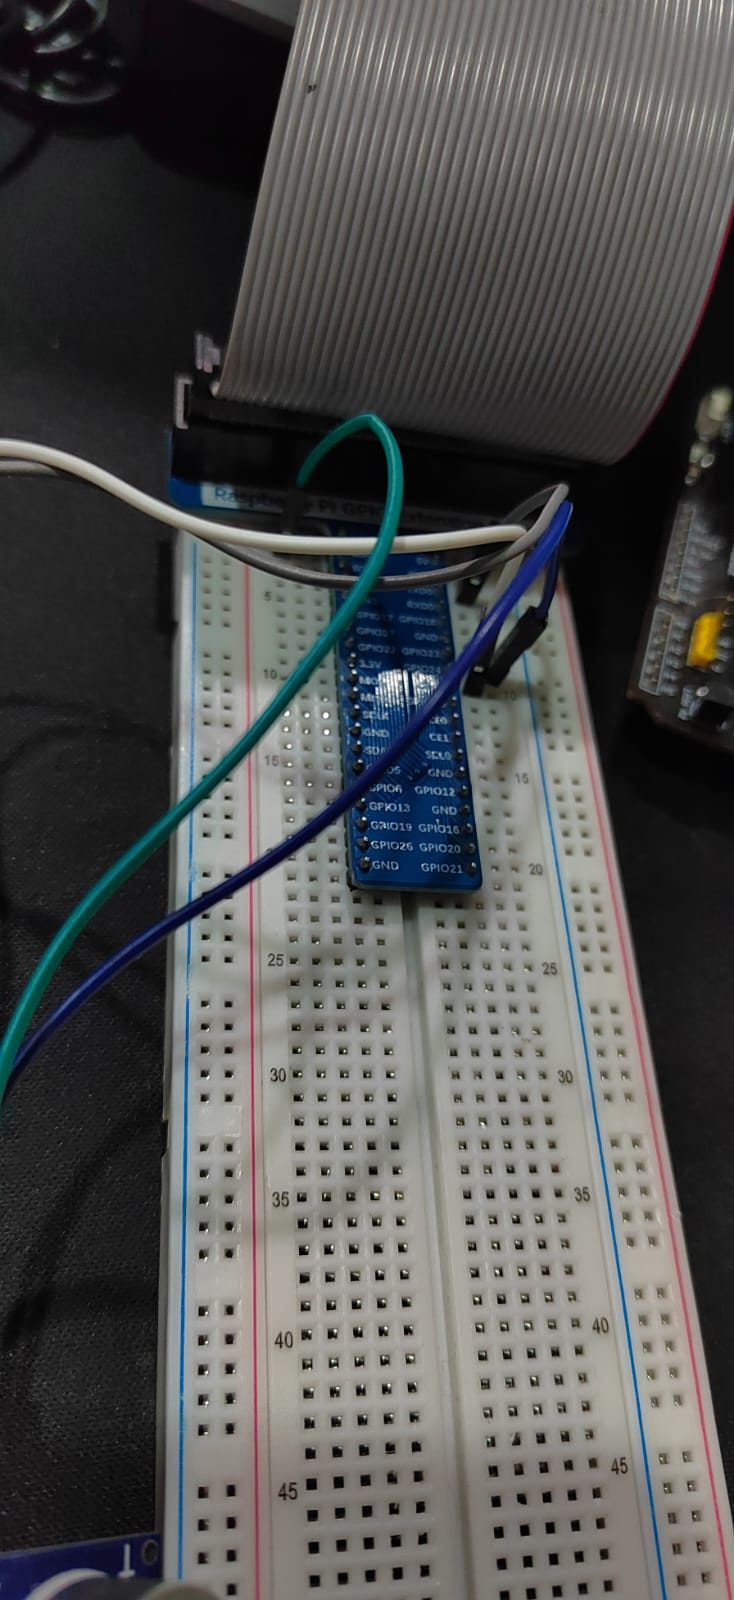
\includegraphics[width=0.5\textwidth]{imagenes/foto1}
	\caption{Foto de las conexiones}
\end{figure}

\begin{figure}[h]
	\centering
	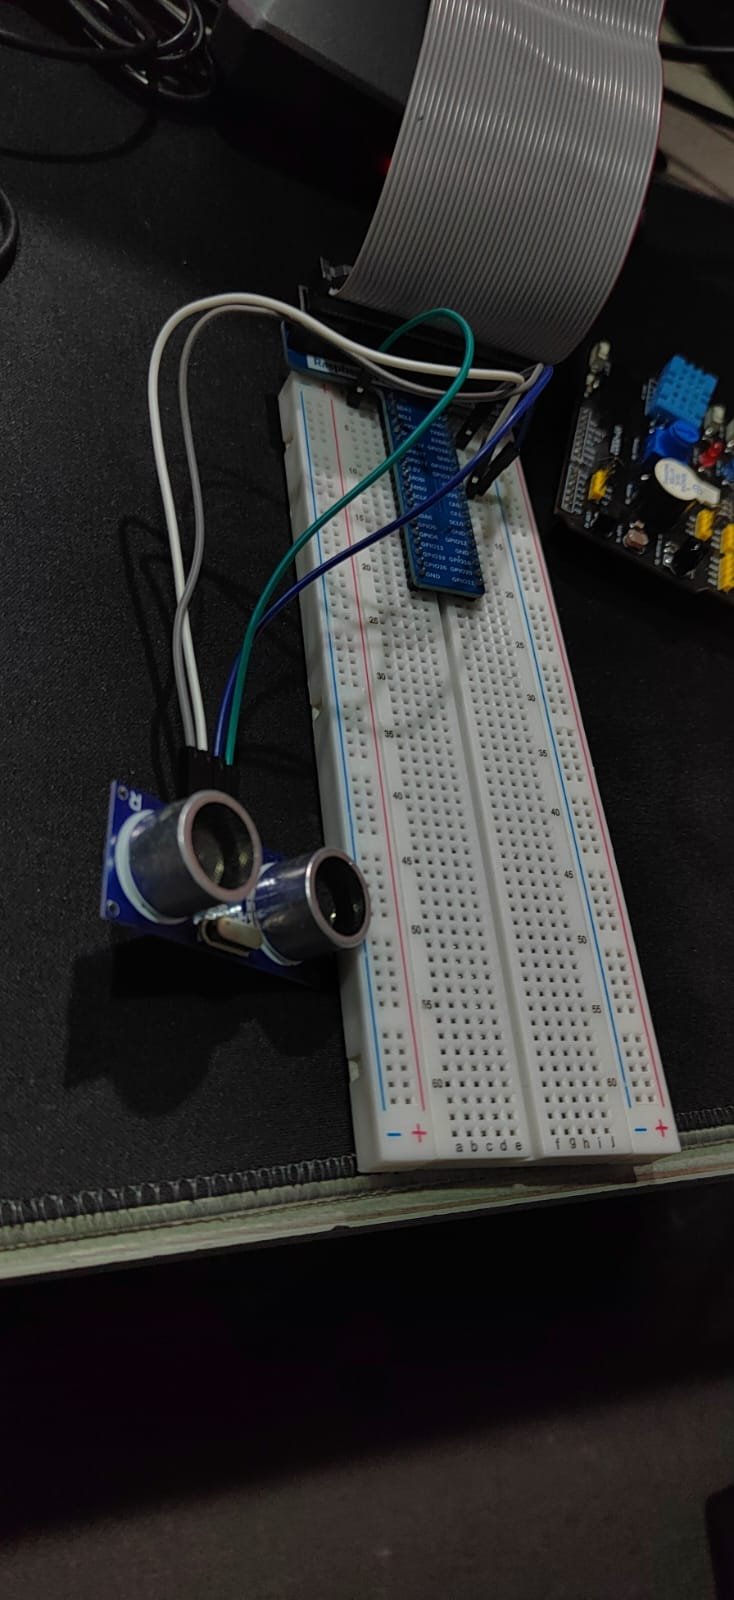
\includegraphics[width=0.5\textwidth]{imagenes/foto2}
	\caption{Divisor de Voltaje}
\end{figure}

\begin{figure}[h]
	\centering
	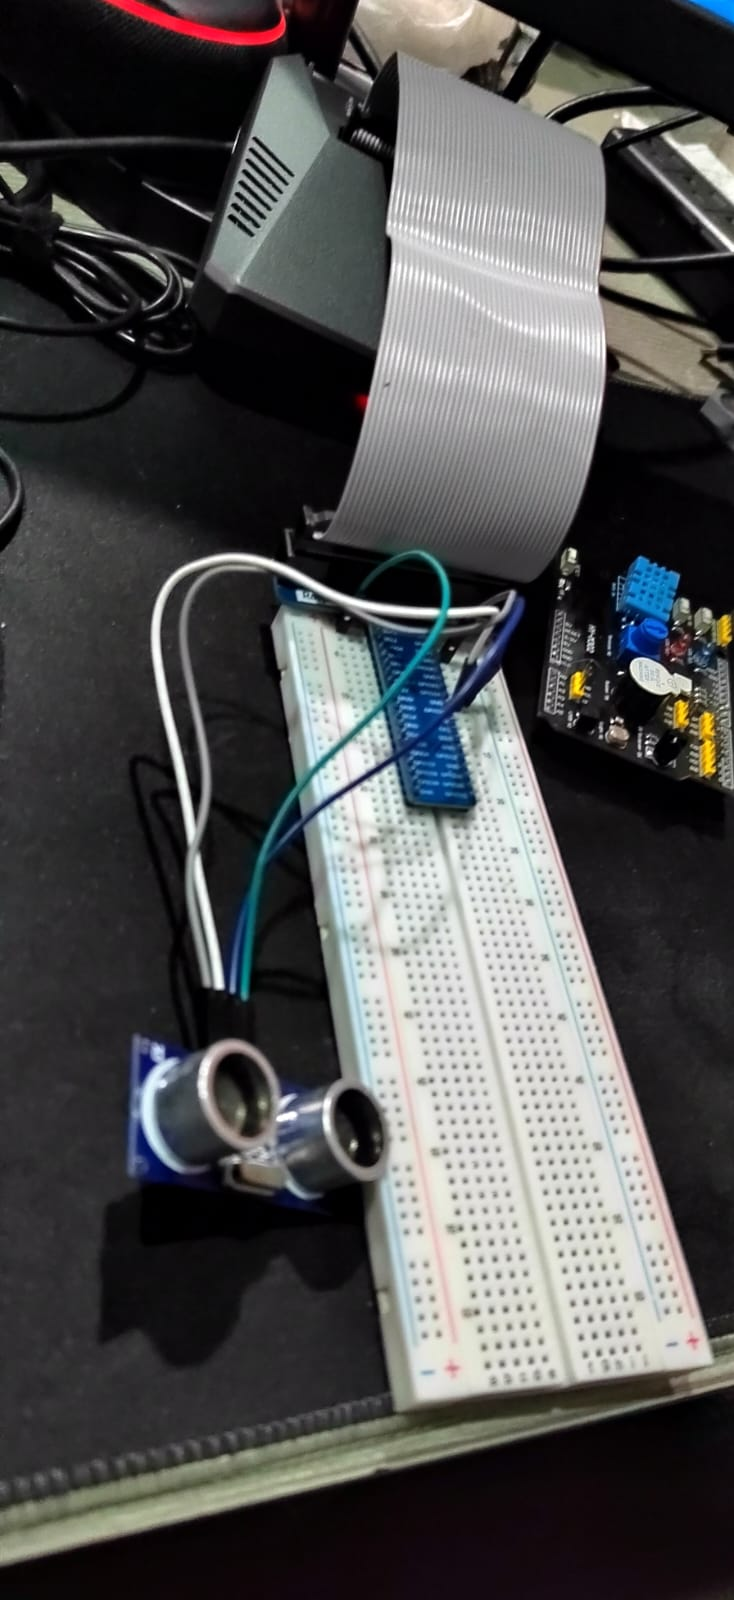
\includegraphics[width=0.5\textwidth]{imagenes/foto3}
	\caption{Conexión Completa}
\end{figure}

	\clearpage
	\section{Conclusión}

Se ha logrado el control eficiente de un servomotor, LEDs y un buzzer mediante el uso de una Raspberry Pi. Este proyecto ha demostrado la capacidad de la Raspberry Pi para interactuar con múltiples dispositivos electrónicos y realizar tareas complejas de automatización.

El proceso de diseño, implementación y prueba de este sistema ha permitido adquirir un conocimiento profundo sobre la programación de la Raspberry Pi y su interacción con componentes electrónicos. Este tipo de proyectos resalta la importancia de la integración de hardware y software, mostrando cómo pueden colaborar para crear soluciones efectivas y funcionales.
	
	% Referencias
	%\clearpage
	%\addcontentsline{toc}{section}{Referencias}
	%\bibliography{referencias} 
	
\end{document}